%! AP Statistics — Unit 3, Lesson 3.6 — Student Guided Notes
\documentclass[10pt]{article}
\usepackage{apstats-article}
\usepackage{apstats-boxes}

\begin{document}

\pageheader{Unit 3, Lesson 3.6}{Guided Notes}
\namedateperiod

\vspace{0.12in}

\begin{objectivebox}
\small By the end of this lesson, I will be able to\dots\\[4pt]
\writeline\\[1pt]
\writeline\\[1pt]
\writeline
\end{objectivebox}

\vspace{0.1in}

\begin{vocabbox}
\termblanklong{Completely randomized design (CRD)}
\termblanklong{Block design}
\termblanklong{Blocking variable / nuisance variable}
\termblanklong{Matched pairs design}
\termblanklong{Precision (in experiments)}
\end{vocabbox}

\vspace{0.1in}

\begin{notesbox}{Choosing an Experimental Design (VAR-3.D)}
\small
\renewcommand{\arraystretch}{2.1}
\begin{tabularx}{\linewidth}{@{} >{\bfseries\color{navy}}p{0.20\linewidth}
    >{\raggedright\arraybackslash}p{0.26\linewidth}
    >{\raggedright\arraybackslash}p{0.25\linewidth}
    >{\raggedright\arraybackslash}X @{}}
\textbf{Design} & \textbf{When to use} & \textbf{Advantage} & \textbf{Limitation} \\
\hline
CRD &
Units are \blank{3cm}; no nuisance variable known &
Simple; maximally random &
\blank{4cm} if a nuisance variable exists \\
Block design &
A nuisance variable is \blank{3cm} and \blank{3cm} &
Removes variability due to the \blank{3cm} variable; increases \blank{2cm} &
Requires knowing the \blank{3cm} in advance \\
Matched pairs &
Units can be \blank{3cm} on a key variable, or same unit can receive both treatments &
Maximum \blank{3cm} of individual differences &
Often requires \blank{3cm} sample; logistics can be complex \\
\end{tabularx}
\end{notesbox}

\vspace{0.1in}

\begin{notesbox}{Decision Framework}
\small
\begin{enumerate}[leftmargin=1.5em, itemsep=8pt]
  \item \textbf{Is there a known variable that affects the response?}\\
        YES $\to$ go to step 2. \quad NO $\to$ use \blank{3cm}.
  \item \textbf{Can units be paired (or can the same unit get both treatments)?}\\
        YES $\to$ use \blank{3cm}. \quad NO $\to$ use \blank{3cm}.
\end{enumerate}

\vspace{6pt}
\textbf{Diagram of a block design:}

\vspace{6pt}
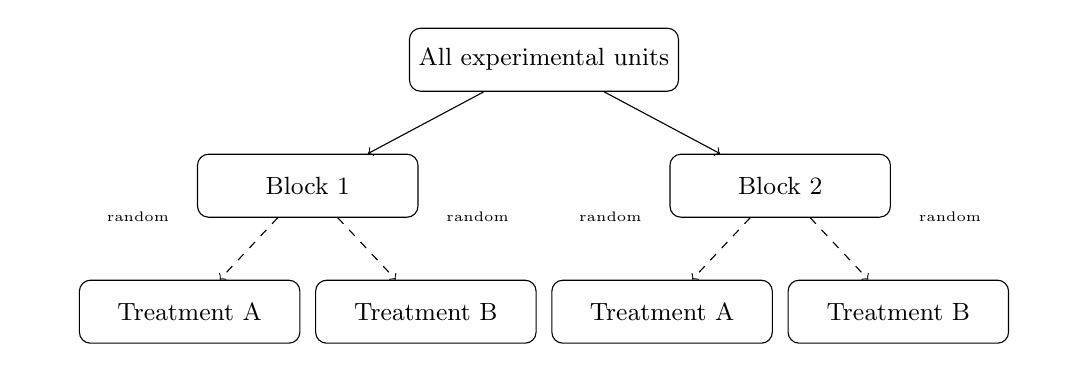
\begin{tikzpicture}[every node/.style={draw, rounded corners, minimum height=0.8cm,
    minimum width=2.8cm, font=\small, align=center}]
  \node (all) at (0,0) {All experimental units};
  \node (b1) at (-3,-1.6) {Block 1};
  \node (b2) at (3,-1.6) {Block 2};
  \node (t1a) at (-4.5,-3.2) {Treatment A};
  \node (t1b) at (-1.5,-3.2) {Treatment B};
  \node (t2a) at (1.5,-3.2) {Treatment A};
  \node (t2b) at (4.5,-3.2) {Treatment B};
  \draw[->] (all) -- (b1);
  \draw[->] (all) -- (b2);
  \draw[->, dashed] (b1) -- node[draw=none, above left, font=\tiny]{random} (t1a);
  \draw[->, dashed] (b1) -- node[draw=none, above right, font=\tiny]{random} (t1b);
  \draw[->, dashed] (b2) -- node[draw=none, above left, font=\tiny]{random} (t2a);
  \draw[->, dashed] (b2) -- node[draw=none, above right, font=\tiny]{random} (t2b);
\end{tikzpicture}
\end{notesbox}

\vspace{0.1in}

\begin{practicebox}
\small A researcher tests two fertilizers on 24 tomato plants. The plants are spread
across 4 greenhouses (6 plants each), and soil quality varies by greenhouse.
\begin{enumerate}[leftmargin=1.5em, itemsep=6pt]
  \item What design should she use? \blank{6cm}
  \item What is the blocking variable? \blank{6cm}
  \item Draw a diagram showing how the 24 plants are assigned.
  \vspace{1.5in}
\end{enumerate}
\end{practicebox}

\end{document}
